\section{Design}\insertloftspace
\setcounter{figure}{0}\setcounter{table}{0}
\label{Des}
\subsection{Brainstorming}
\label{BraSto}
Right after we defined the project, we took some time to propose ideas. The goal was to abstract from the existing and imagine different configurations, shapes, or mechanisms. So we made hand sketches to illustrate our different ideas as shown in the drawings below. 
\begin{figure}[H]
    \begin{subfigure}{.5\linewidth}
        \centering
        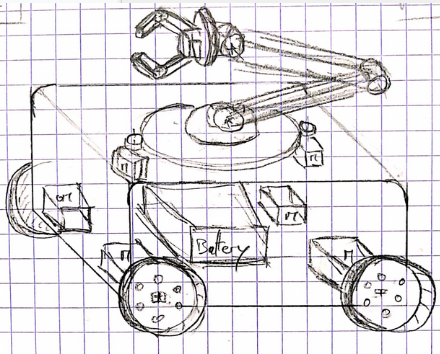
\includegraphics[scale = 0.3]{Images/Section03/Drawing1.png}
        \caption{}
        \label{fig:Drawing1}
    \end{subfigure}%
    \begin{subfigure}{.5\linewidth}
        \centering
        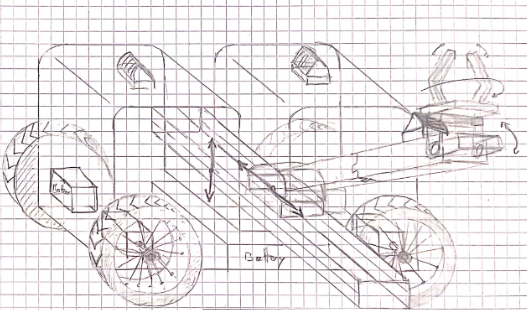
\includegraphics[scale = 0.3]{Images/Section03/Drawing2.png}
        \caption{}
        \label{fig:Drawing2}
    \end{subfigure}\\[1ex]
    \begin{subfigure}{.5\linewidth}
        \centering
        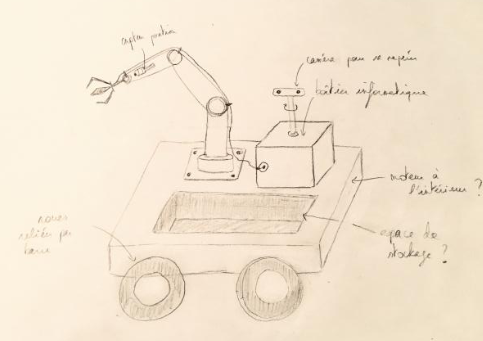
\includegraphics[scale = 0.3]{Images/Section03/Drawing3.png}
        \caption{}
        \label{fig:Drawing3}
    \end{subfigure}
    \begin{subfigure}{.5\linewidth}
        \centering
        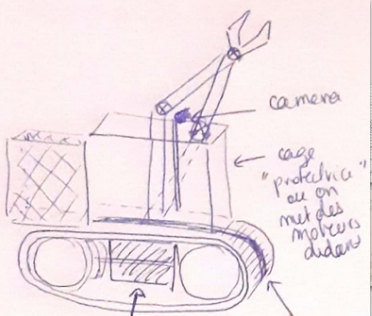
\includegraphics[scale = 0.3]{Images/Section03/Drawing4.png}
        \caption{}
        \label{fig:Drawing4}
    \end{subfigure}
    \caption{Robot drawings}
    \label{fig:Drawings}
\end{figure}

In order to prototype and select a design quickly we also built two lego prototypes. This allowed us to define the basic design of the arm: a three-degree-of-freedom arm attached with a pivot link to the base. We hesitated with the design of the figure \ref{fig:Drawing2} with a central axis but when we built the lego prototype we found constraints too important to reach different points in space. In particular, the ability to work only in a 2D plane without moving the base.
\begin{figure}[H]
    \begin{subfigure}{.5\linewidth}
        \centering
        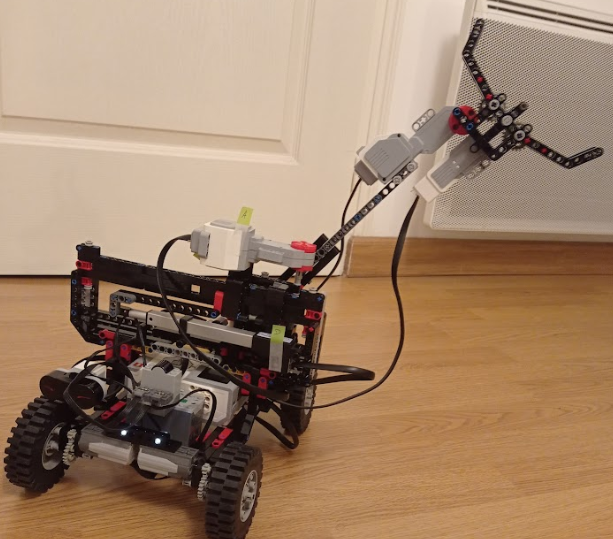
\includegraphics[scale = 0.2]{Images/Section03/Lego1.png}
        \caption{}
        \label{fig:Lego1}
    \end{subfigure}%
    \begin{subfigure}{.5\linewidth}
        \centering
        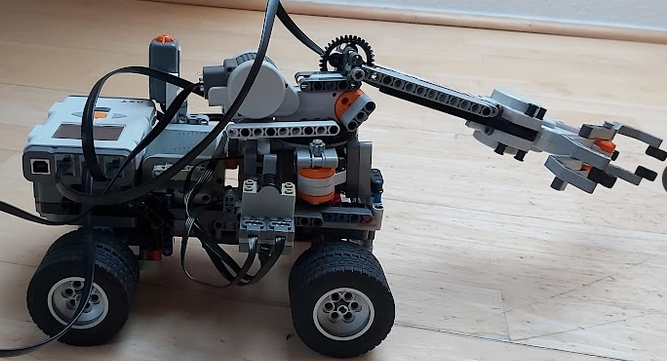
\includegraphics[scale = 0.3]{Images/Section03/Lego2.png}
        \caption{}
        \label{fig:Lego2}
    \end{subfigure}\\[1ex]
    \caption{Lego robots}
    \label{fig:Legos}
\end{figure}

Like the market research and project definition, all members participated in this step in order to get as many ideas as possible but also to be sure everyone understand the future goal. We then divided ourselves into technical divisions as detailed in the previous \ref{Orga}. Once this process was finished, the mechanical pole could start a design in \gls{CAD}\footnote{the use of computers to aid in the creation, modification, analysis, or optimization of a design} using the software \textit{Onshape}.

\subsection{Onshape}
\label{Ons}
\subsubsection{Presentation}

To model our robot, we used the software \textit{Onshape} \cite{Onshape}. It is a computer-aided design software system, delivered over the Internet via a software-as-a-service model. This software offers many advantages : 
\begin{itemize}[noitemsep]
    \item collaborative
    \item quick to learn
    \item online
\end{itemize}

The last one may limit its use because it requires an internet connection.

\subsubsection{Rules}

Rules to standardize our work have also been established from the beginning. As we will see in the following parts, it is necessary to respect them to be able to exploit these documents with other software.
\begin{itemize}
    \item Name all parts with a specific name: it is the ID of the part and it has to be unique
    \item One subassembly by articulation: a subassembly contains all the parts of an articulation that have a fixed join between them
    \item One main assembly containing the motor links: the main assembly contains only the join that you want to see at the end. Usually, it is the dynamic join but it can be fixed to get a part separately.
    \item Assign material to each part: in \textit{Onshape}, you precise the volumic mass, you need to pay attention in case you use PLA with a 3D printer. A part is never full at 100\% and you need to adapt the volumic mass to get the correct masS.
    \item Motor link in the main assembly needs to be named \textit{dof\_\less link\_name\bg}
    \item A relation between parent/child needs to be respected for every link: In \textit{Onshape}, like all CAO software, there is a parent/child relation in every link. You need to pay attention to this, it can be a source of many errors if you want to export your model. When you create a link, fixed or motorized, the first element you click on is the child. The second one is the father. You can then check the parent and the child as shown in the following image. It is therefore necessary to start from the origin to the end of the robot, respecting these relationships at the time of assembly.
\end{itemize}
\begin{figure}[H]
    \centering
    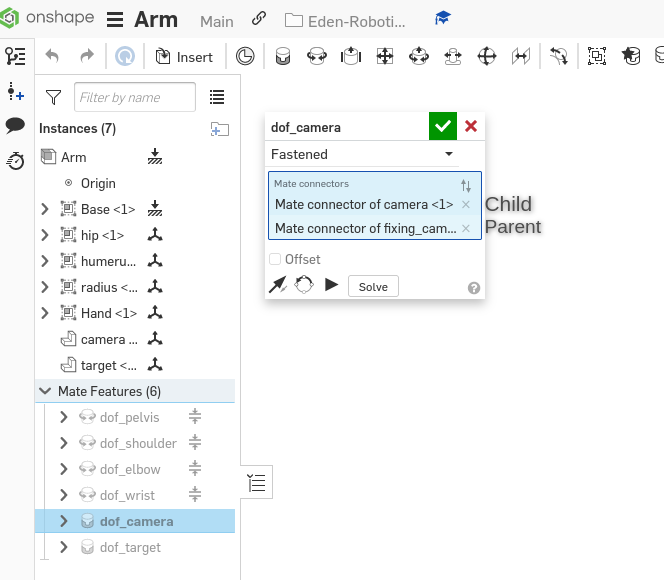
\includegraphics[width=0.5\textwidth]{Images/Section03/Parent_Child.png}
    \caption{Parent child principle}
    \label{fig:ParentChild}
\end{figure}

\subsection{Arm}
\label{Arm}
The design of the arm was done in 4 steps.

\subsubsection{Step 1}

For the first step, we looked for and bought an arm resembling the desired design. Thanks to this, the mechanical department was able to train on different tutorials and then to make an "easy" application that consisted only in reproducing this arm by respecting the rules stated. At the same time, the automatic pole was able to take advantage of this to make tests on a physical robot.
\begin{figure}[H]
    \begin{subfigure}{.5\linewidth}
        \centering
        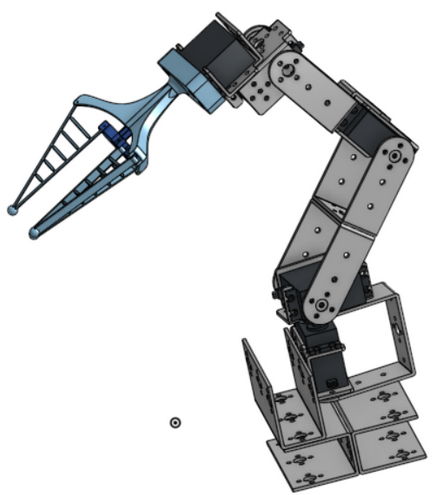
\includegraphics[scale = 0.2]{Images/Section03/prototype_onshape1.png}
        \caption{Onshape design}
        \label{fig:Onshape1}
    \end{subfigure}%
    \begin{subfigure}{.5\linewidth}
        \centering
        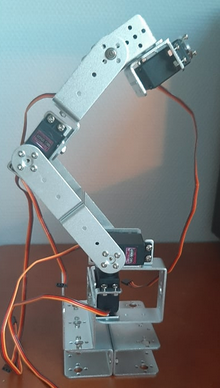
\includegraphics[scale = 0.3]{Images/Section03/prototype1.png}
        \caption{Physical robot}
        \label{fig:Physical1}
    \end{subfigure}\\[1ex]
    \caption{Prototype 1}
    \label{fig:Prototype1}
\end{figure}

The purchase of this arm allowed a first quick design on which all the members could work. We thus avoided a waiting time for the computer science and automatic poles. They were able to work on this one and carry out various tests in order to leave time for the mechanical pole to create our own design that we were going to manufacture.

\subsubsection{Step 2 and 3}

In steps 2 and 3, we created different prototypes entirely on the computer. Little manufacturing was done, we only tested parts of the robot in order to save time and iterate as quickly as possible.
\begin{figure}[H]
    \begin{subfigure}{.5\linewidth}
        \centering
        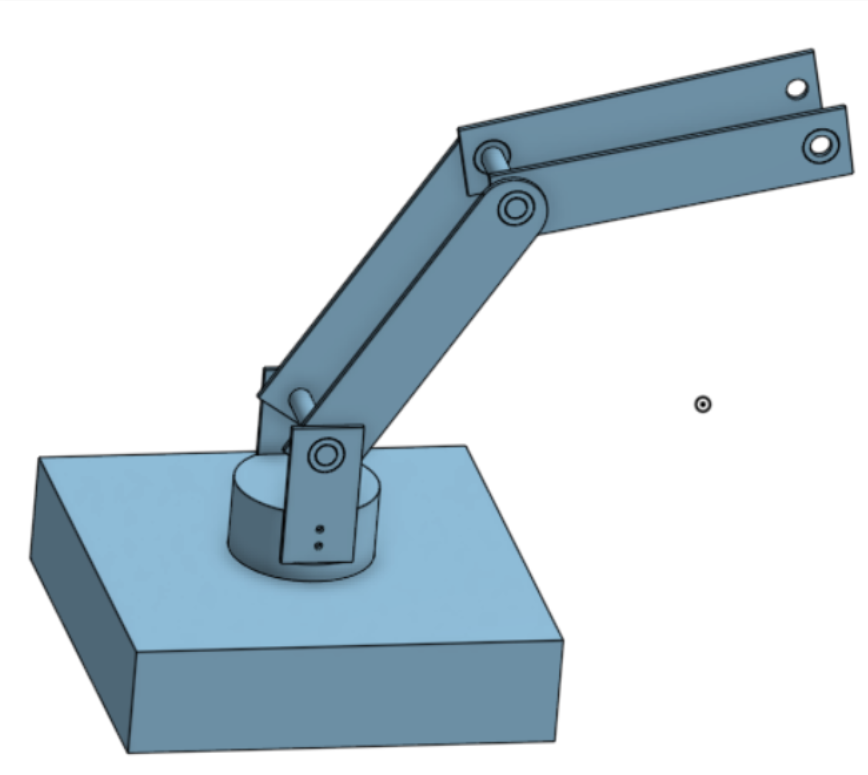
\includegraphics[scale = 0.3]{Images/Section03/prototype2.png}
        \caption{Prototype 2}
        \label{fig:Prototype2}
    \end{subfigure}%
    \begin{subfigure}{.5\linewidth}
        \centering
        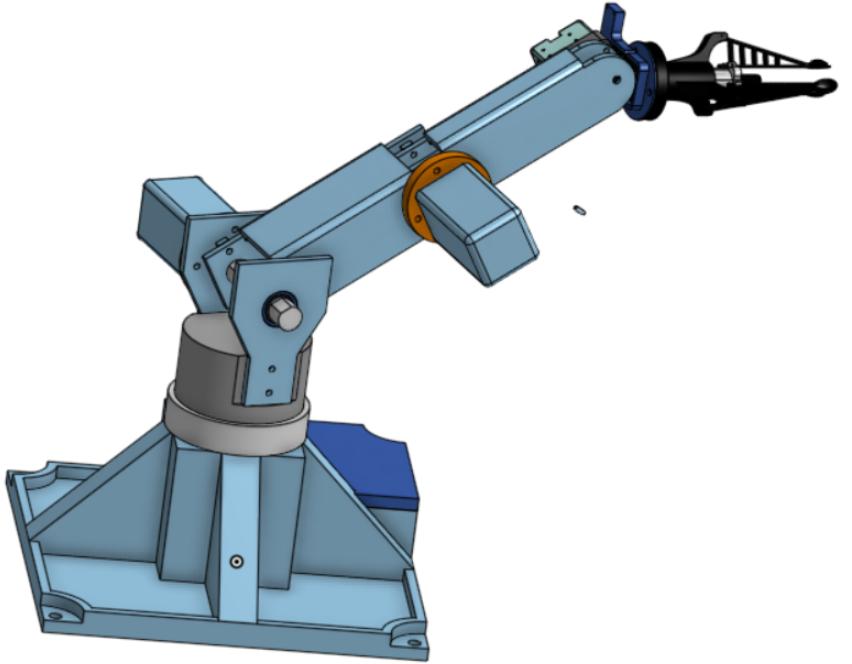
\includegraphics[scale = 0.3]{Images/Section03/prototype3.png}
        \caption{Prototype 3}
        \label{fig:Prototype3}
    \end{subfigure}\\[1ex]
    \caption{Prototypes 2 and 3}
    \label{fig:Prototypes}
\end{figure}

Prototype 2 was a rough sketch of our robot. As we said, we decided to have 3 degrees of freedom on the arm (shoulder, elbow, wrist) and a pivot link on the base to reach a maximum of points in space. We can thus have a base that will settle in one place and an arm that will recover a maximum of tomatoes without having to move it. In view of the layout of the tomatoes, we also decided to have two parts that we will call humerus and radius almost the same size. 

\bigbreak
It allowed us to make choices like the types of joints, and the lengths of each of the parts. Some of us also followed the training courses offered by Centrale on 3D printing and laser cutting. Some parts of this design, although rough, have been created to practice.
\begin{figure}[H]
    \begin{subfigure}{.5\linewidth}
        \centering
        \includegraphics[scale = 0.5]{Images/Section03/3D\_printed1.png}
        \caption{3D printed part}
        \label{fig:3D1}
    \end{subfigure}%
    \begin{subfigure}{.5\linewidth}
        \centering
        \includegraphics[width= 0.9\textwidth,scale = 0.3]{Images/Section03/laser\_cutting1.png}
        \caption{Laser cutting part}
        \label{fig:LC1}
    \end{subfigure}\\[1ex]
    \caption{3D printed and laser cutting examples}
    \label{fig:3DLC1}
\end{figure}

We then designed another robot (step 3) more complete since it integrates the wrist mechanism. The motors and the ball bearings were also represented, with realistic masses. Following the problems we noticed during the manufacturing of some parts, we also imagined a new structure for the arms to stiffen the whole. However, the geometry implied a one-piece construction of the arm rather than two laser-cut parts. It had to be 3D printed, which increased the production time. Although the structure was better bonded, these parts also lacked strength at the corners. It was therefore not retained.
\begin{figure}[H]
    \centering
    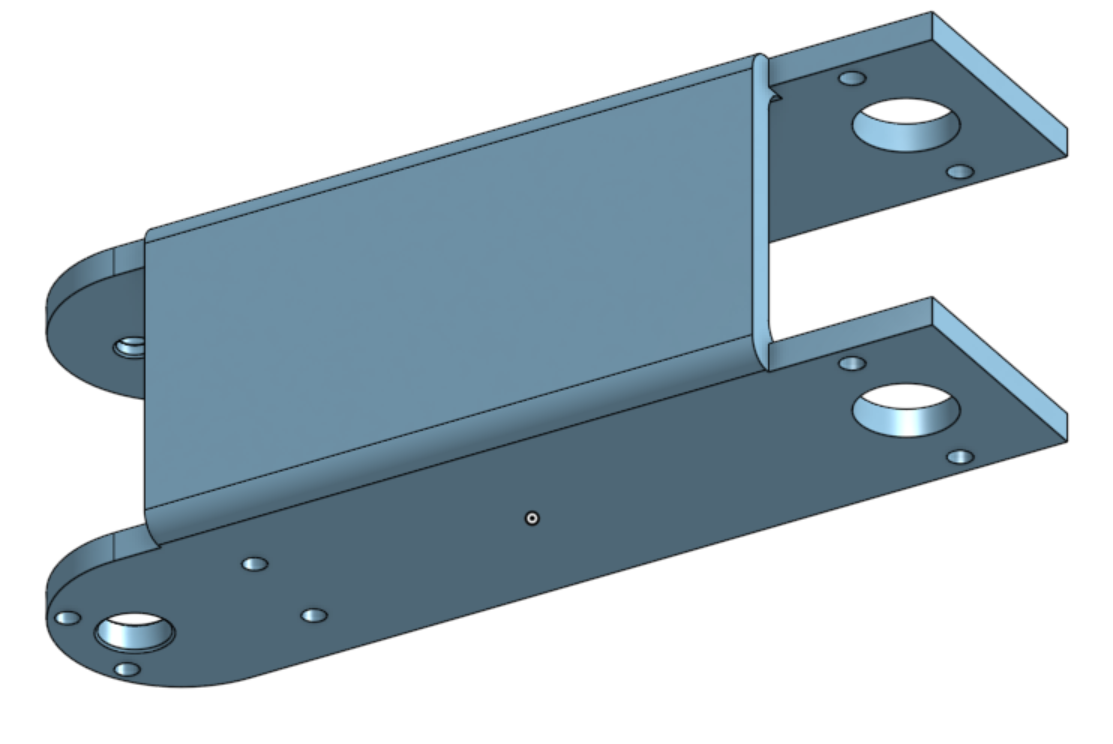
\includegraphics[width=0.5\textwidth]{Images/Section03/Arm2.png}
    \caption{Arm modified}
    \label{fig:Arm2}
\end{figure}

It is on this robot that the studies of part 6 were led first to select the motors for the final robot. 

\subsubsection{Step 4}

All these tests and changes lead us to step 4: the complete design of the robot and its complete fabrication. For this, we made some parts in PVC or plywood with a laser cut, we printed in 3D some parts. Others such as the filleted rods were directly purchased. To overcome the lack of rigidity, we added rods between the two plates of the humerus and radius. A building instruction to reproduce the robot can be found in appendix \ref{Instructions}. All the STL files can also be found on the GitHub page of this project.
\begin{figure}[H]
    \begin{subfigure}{.5\linewidth}
        \centering
        \includegraphics[scale = 0.5]{Images/Section03/partial\_assembly.png}
        \caption{Partial assembly}
        \label{fig:PA}
    \end{subfigure}%
    \begin{subfigure}{.5\linewidth}
        \centering
        \includegraphics[width= 0.6\textwidth,scale = 0.8]{Images/Section03/final\_assembly.png}
        \caption{Final assembly}
        \label{fig:FA}
    \end{subfigure}\\[1ex]
    \caption{Arm step 4}
    \label{fig:AS4}
\end{figure}

This is only a prototype and improvements are still to be expected. We had some ideas that we, unfortunately, could not explore. Some PVC parts can be replaced by aluminum to increase the resistance, and a structure around the arm to manage the cables can also be added for example.

\subsection{Hand}
\label{Han}

The design of the hand was a crucial step. Based on what was being done and the advantages put forward, we created our own design. The two figures below present techniques to catch objects, one based on aspiration\cite{Abundant} and the other mimicking a human hand\cite{Prehenseur}. However, the first one is relatively complex and therefore expensive and long to implement. Moreover, there is a risk of damaging the fruit by sucking it too hard. The second one is not very adapted for tomatoes. 
\begin{figure}[H]
    \begin{subfigure}{.5\linewidth}
        \centering
        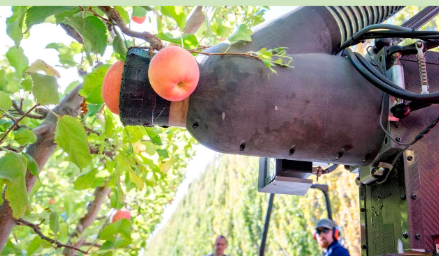
\includegraphics[scale = 0.7]{Images/Section03/hand1.png}
        \caption{Hand 1}
        \label{fig:hand1}
    \end{subfigure}%
    \begin{subfigure}{.5\linewidth}
        \centering
        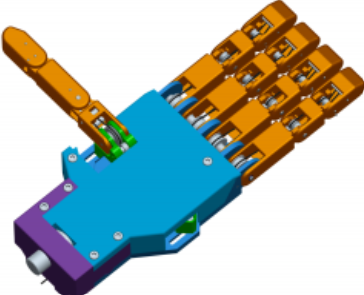
\includegraphics[width= 0.6\textwidth,scale = 0.8]{Images/Section03/hand2.png}
        \caption{Hand 2}
        \label{fig:hand2}
    \end{subfigure}\\[1ex]
    \caption{Existing hands}
    \label{fig:ExistingHands}
\end{figure}

Our first idea was to create a hand composed of three deformable rights that would follow the shape of the tomato. These fingers are attached to a fixed part and to the same actuator to make them move at the same time. The actuator is a screw-nut system and an adapter to make the 3D-printed fingers move.
\begin{figure}[H]
    \begin{subfigure}{.5\linewidth}
        \centering
        \includegraphics[scale = 0.6]{Images/Section03/hand\_proto1.png}
        \caption{Onshape design}
        \label{fig:HandProto1}
    \end{subfigure}%
    \begin{subfigure}{.5\linewidth}
        \centering
        \includegraphics[scale = 0.6]{Images/Section03/hand\_proto_real1.png}
        \caption{Hand}
        \label{fig:HProtoReal1}
    \end{subfigure}\\[1ex]
    \begin{subfigure}{\linewidth}
        \centering
        \includegraphics[width=0.4\textwidth]{Images/Section03/hand\_system.png}
        \caption{Actuator system}
        \label{fig:HSystem}
    \end{subfigure}
    \caption{Hand V1}
    \label{fig:HandV1}
\end{figure}

Unfortunately, with our knowledge and facing the difficulty to find a material deformable enough to fit the shape of the tomato while supporting enough to pull it, we changed the shape of the fingers. While keeping the principle of three fingers, they have been adapted to have a spoon shape and come directly into the shape of the tomato.
\begin{figure}[H]
    \begin{subfigure}{.5\linewidth}
        \centering
        \includegraphics[scale = 0.7]{Images/Section03/hand\_picking.png}
        \caption{Hand picking tomato}
        \label{fig:HandPicking}
    \end{subfigure}%
    \begin{subfigure}{.5\linewidth}
        \centering
        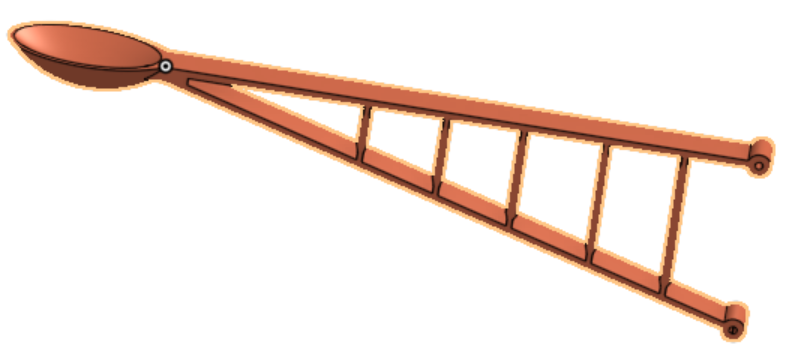
\includegraphics[scale=0.5]{Images/Section03/finger1.png}
        \caption{Finger}
        \label{fig:Finger}
    \end{subfigure}\\[1ex]
    \caption{Hand V2}
    \label{fig:HandV2}
\end{figure}

This requires greater precision when picking the fruit, however. This configuration also offers less flexibility when it comes to the different shapes of tomatoes. It could be interesting to try to pursue the principle of a deformable hand. 